\chapter{Results}
This chapter discusses the results we obtained by processing data on HCP pipelines. The differences we observed and the quantified metric values are discussed in detail for each pipeline. Section \ref{sec:Prefreesurfer} discusses PrefreeSurfer results, followed by section \ref{sec:Freesurfer} on FreeSurfer results, section \ref{sec:Postfreesurfer} on PostFreeSurfer results and last section \ref{sec:fMRI} discusses fMRIVolume pipeline results.

\section{PreFreeSurfer} \label{sec:Prefreesurfer}
The subjects were processed on CentOS6 and CentOS7 using the PreFreeSurfer pipeline. Among the 92 NIFTI imaging files common to all 5 subjects, 76 (.nii.gz) files differed between CentOS6 and CentOS7. Figure~\ref{fig:prefreesurfer_metric_values} shows the Dice coefficient value and NRMSE values of the nifti files that were found to have differences in between operating systems. The mean, median and standard deviation NRMSE and Dice coefficient values are given in Table~\ref{tab:PreFreeSurfer_Metic_Values}.

\hfill \break
\begin{center}
\begin{tabular}{|l|l|l|}
\hline
\textbf{Item}      & \textbf{Nrmse} & \textbf{Dice} \\ \hline
Mean               & 0.006998923    & 0.229517835   \\ \hline
Median             & 0.003744135    & 0.02166149    \\ \hline
Standard Deviation & 0.013993721    & 0.337104803   \\ \hline
\end{tabular}
\captionof{table}{NRMSE \& DICE values for PreFreeSurfer processing on CentOS6 and CentOS7}
\label{tab:PreFreeSurfer_Metic_Values}
\end{center}
\hfill \break

\begin{center}
\begin{longtable}{|p{.3\textwidth}|p{.3\textwidth}|p{.3\textwidth}|}
\cline{1-3}
\textbf{Category} & \textbf{Nrmse} & \textbf{Dice Coeff} \\\cline{1-3}
\multirow{5}{.2\textwidth}{Files consistently different across subjects (low std.dev)}     & \makecell[l]{NonlinearIntensities.nii.gz \\ (BrainExtraction\\\_FNIRTbased)}  & \makecell[l]{T1w\_acpc\_to\_MNI\\\_roughlin.nii.gz \\ (BrainExtraction\\\_FNIRTbased)} \\\cline{2-3}
& \makecell[l]{sqrtT1wbyT2w.nii.gz \\(T2wToT1wDistortion\\CorrectAndReg)}                   & \makecell[l]{NonlinearIntensities.nii.gz\\(BrainExtraction\\\_FNIRTbased)} \\\cline{2-3}
& \makecell[l]{NonlinearReg.nii.gz\\(BrainExtraction\\\_FNIRTbased)}                        & \makecell[l]{NonlinearReg\\Jacobians.nii.gz\\(xfms)} \\\cline{2-3}
& \makecell[l]{FieldMap2T1w\_acpc.nii.gz\\(T2wToT1wDistortion\\CorrectAndReg)}              & \makecell[l]{T2w\_acpc.nii.gz\\(T2wToT1wDistortion\\CorrectAndReg)} \\\cline{2-3}
& \makecell[l]{T1w\_acpc\_dc\_brain.nii.gz\\(T1w)}                                        & \makecell[l]{T1w.nii.gz\\(MNINonLinear)} \\\cline{1-3}
\multirow{5}{.2\textwidth}{Files with differences that vary across subjects (med std. dev)} & \makecell[l]{T2w\_restore.nii.gz\\(MNINonLinear)}  & \makecell[l]{T1w\_acpc\_dc\_brain.nii.gz\\(T1w)} \\\cline{2-3}
& \makecell[l]{acpc\_final.nii.gz \\(ACPCAlignment)}                       & \makecell[l]{T1wmulT2w\_brain \\ \_norm\_modulate.nii.gz\\(BiasFieldCorrection\\\_sqrtT1wXT1w)} \\\cline{2-3}
& \makecell[l]{T1w\_dc.nii.gz\\(xfms)}                           & \makecell[l]{T1w\_dc.nii.gz\\(xfms)} \\\cline{2-3}
& \makecell[l]{T1w\_acpc\_dc.nii.gz\\(T1w)}                      & \makecell[l]{T2w\_acpc\_to \\ \_MNI\_nonlin.nii.gz\\(BrainExtraction\\\_FNIRTbased)} \\\cline{2-3}
& \makecell[l]{T1w\_acpc.nii.gz\\(T2wToT1wDistortion\\CorrectAndReg)}  & \makecell[l]{T1wmulT2w\_brain\\\_norm\_s5.nii.gz\\(BiasFieldCorrection\\\_sqrtT1wXT1w)} \\\cline{1-3}
\multirow{5}{.2\textwidth}{Files with differences that vary specific to each subject (large std. dev)}   & \makecell[l]{acpc\_final.nii.gz\\(ACPCAlignment)}  & \makecell[l]{acpc\_final.nii.gz\\(ACPCAlignment)} \\\cline{2-3}
& \makecell[l]{T1w\_acpc\_to \\ \_MNI\_roughlin.nii.gz\\(BrainExtraction\\\_FNIRTbased)}                 & \makecell[l]{NonlinearIntensities.nii.gz\\(BrainExtraction\\\_FNIRTbased)} \\\cline{2-3}
& \makecell[l]{T2w.nii.gz\\(T2w)}                                                            & \makecell[l]{FieldMap2T1w\_acpc \\ \_ShiftMap.nii.gz\\(T2wToT1wDistortion\\CorrectAndReg)} \\\cline{2-3}
  & \makecell[l]{T1wmulT2w\_brain \\ \_norm\_s5.nii.gz\\(BiasFieldCorrection\\\_sqrtT1wXT1w)}                   & \makecell[l]{bias\_raw.nii.gz\\(BiasFieldCorrection\\\_sqrtT1wXT1w)} \\\cline{2-3}
  & \makecell[l]{T2w\_dc\_reg.nii.gz\\(T2wToT1wDistortion\\CorrectAndReg)}                                                   & \makecell[l]{FieldMap2T1w\_acpc.nii.gz\\(T2wToT1wDistortion\\CorrectAndReg)} \\\cline{1-3}
\end{longtable}
\captionof{table}{NRMSE \& DICE comparison of PreFreeSurfer files with differences on CentOS6 and CentOS7}
\label{tab:PreFreeSurfer_comparison_table}
\end{center}
\hfill \break

\hfill \break
\begin{center}
\begin{tabular}{|l|l|}
\hline
\textbf{Process}      & \textbf{Filename} \\ \hline
T2wToT1wDistortionCorrectAndReg               & FieldMap2T1w\_acpc.nii.gz    \\ \hline
MNINonLinear             & NonlinearIntensities.nii.gz    \\ \hline
BrainExtraction\_FNIRTbased & NonlinearRegJacobians.nii.gz   \\ \hline
BrainExtraction\_FNIRTbased & standard2str.nii.gz \\ \hline
T2wToT1wDistortionCorrectAndReg & T2w\_dc\_reg.nii.gz \\ \hline
T2wToT1wDistortionCorrectAndReg & sqrtT1wbyT2w.nii.gz \\ \hline
\end{tabular}
\captionof{table}{Processes and corresponding files with the top mean to std. dev ratio (NRMSE)}
\label{tab:PreFreeSurfer_NRMSE_processes}
\end{center}
\hfill \break

\hfill \break
\begin{center}
\begin{tabular}{|l|l|}
\hline
\textbf{Process}      & \textbf{Filename} \\ \hline
T1w              & T1w\_acpc\_dc\_brain.nii.gz    \\ \hline
BiasFieldCorrection\_sqrtT1wXT1w             & \makecell[l]{T1wmulT2w\_brain\\\_norm\_modulate.nii.gz}    \\ \hline
T2wToT1wDistortionCorrectAndReg & FieldMap2T2w\_acpc\_Warp.nii.gz   \\ \hline
MNINonLinear & \makecell[l]{T1w\_acpc\_dc\_restore\\\_brain\_to\_MNILinear.nii.gz} \\ \hline
BrainExtraction\_FNIRTbased & NonlinearIntensities.nii.gz \\ \hline
BiasFieldCorrection\_sqrtT1wXT1w & T1wmulT2w.nii.gz \\ \hline
\end{tabular}
\captionof{table}{Processes and corresponding files with the top mean to std. dev ratio (DICE)}
\label{tab:PreFreeSurfer_NRMSE_processes}
\end{center}
\hfill \break

%\begin{center}
%  \begin{tabular}{|p{.30\textwidth}|p{.30\textwidth}|p{.30\textwidth}|}
%  \hline
%  \multirow{3}{.30\textwidth}{looooooong cell} & cell1 & cell2 \\ \cline{2-3}
%   & cell3 & cell4 \\ \cline{2-3}
%   & cell5 & cell6 \\ \hline
%\end{tabular}
%\end{center}
%\hfill \break

\begin{center}
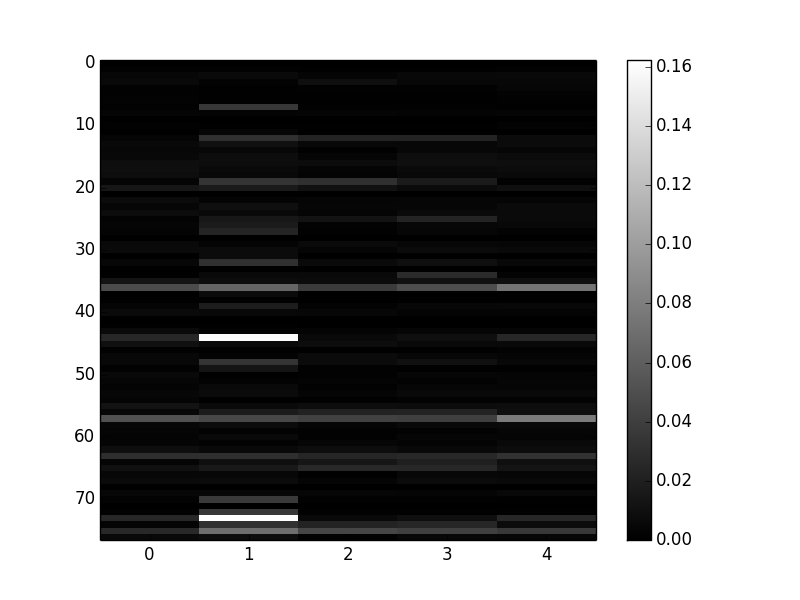
\includegraphics[width=.5\linewidth]{prefreesurfer_nrmse.png}%
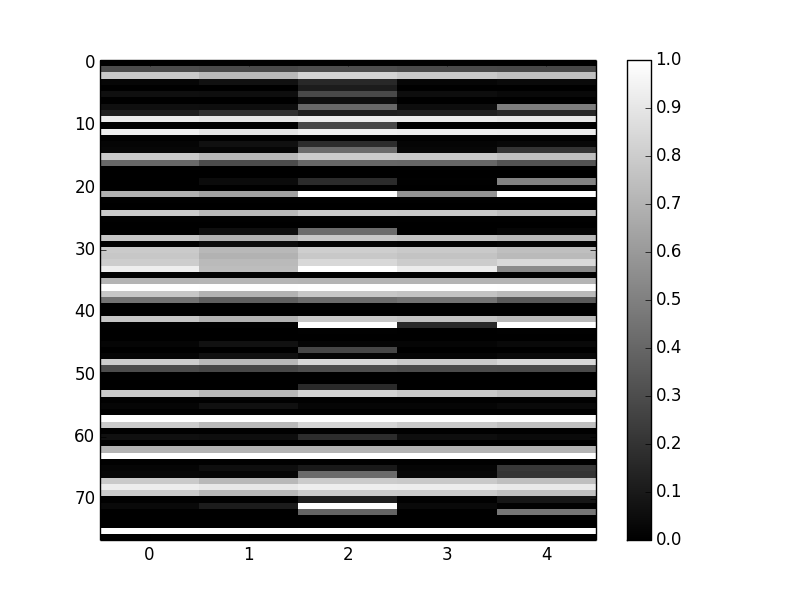
\includegraphics[width=.5\linewidth]{prefreesurfer_dice.png}
\captionof{figure}{PreFreeSurfer metric values}
\caption*{(i) NRMSE (left) (ii)Dice coefficient (right)}
\label{fig:prefreesurfer_metric_values}
\end{center}

\section{FreeSurfer} \label{sec:Freesurfer}
FreeSurfer results presented in this section does not take into account the files that were found to be different in PreFreeSurfer pipeline. The number of files that has differences and which are common to all the subjects, was found to be 61 files (23 .nii.gz files and 38 .mgz files). Table~\ref{tab:FreeSurfer_Metic_Values} contains the details about the mean, median and standard deviation of NRMSE and Dice coefficient values. Figure~\ref{fig:freesurfer_metric_values} illustrates the NRMSE and Dice coefficient values in the form of mat
\hfill \break
\begin{center}
\begin{tabular}{|l|l|l|}
\hline
\textbf{Item}      & \textbf{Nrmse} & \textbf{Dice} \\ \hline
Mean               & 0.017669782    & 0.695379753   \\ \hline
Median             & 0.009735296    & 0.926226795   \\ \hline
Standard Deviation & 0.018183193    & 0.405144714   \\ \hline
\end{tabular}
\captionof{table}{NRMSE \& DICE values for FreeSurfer processing on CentOS6 and CentOS7}
\label{tab:FreeSurfer_Metic_Values}
\end{center}
\hfill \break

\begin{center}
\begin{longtable}{|p{.3\textwidth}|p{.3\textwidth}|p{.3\textwidth}|}
\cline{1-3}
\textbf{Category} & \textbf{Nrmse} & \textbf{Dice Coeff} \\\cline{1-3}
\multirow{5}{.3\textwidth}{Files consistently different across subjects (low std.dev)}     & \makecell[l]{T1w\_hires.greynorm.nii.gz \\ (MRI)}  & \makecell[l]{T2w\_hires.norm.nii.gz\\ (MRI)} \\\cline{2-3}
& \makecell[l]{T1w\_hires.greynorm.mgz\\(MRI)}                   & \makecell[l]{T2w\_hires.norm.mgz\\(MRI)} \\\cline{2-3}
& \makecell[l]{T1w\_hires.greynorm\\\_ribbon.nii.gz\\(MRI)}                        & \makecell[l]{T1w\_acpc\_dc\\\_restore\_1mm.nii.gz\\(T1w)} \\\cline{2-3}
& \makecell[l]{T1w\_hires.nii.gz\\(MRI)}              & \makecell[l]{rawavg.mgz\\(MRI)} \\\cline{2-3}
& \makecell[l]{T1w\_hires.norm.nii.gz\\(MRI)}                                        & \makecell[l]{001.mgz\\(MRI)} \\\cline{1-3}
\multirow{5}{.3\textwidth}{Files with differences that vary across subjects (med std. dev)} & \makecell[l]{aseg.auto\_noCCseg.mgz\\(MRI)}  & \makecell[l]{aparc.a2009s+aseg.mgz\\(T1w)} \\\cline{2-3}
& \makecell[l]{wm.asegedit.mgz\\(MRI)}                       & \makecell[l]{ribbon.nii.gz\\(MRI)} \\\cline{2-3}
& \makecell[l]{wm.mgz\\(MRI)}                           & \makecell[l]{ribbon\_inv.nii.gz\\(MRI)} \\\cline{2-3}
& \makecell[l]{ctrl\_pts.mgz\\(MRI)}                      & \makecell[l]{T1wMulT2w\_hires.nii.gz\\(MRI)} \\\cline{2-3}
& \makecell[l]{aseg.hires.nii.gz\\(MRI)}  & \makecell[l]{aseg.hires.nii.gz\\(MRI)} \\\cline{1-3}
\multirow{5}{.3\textwidth}{Files with differences that vary specific to each subject (large std. dev)}   & \makecell[l]{talairach.m3z.inv.x.mgz\\(MRI)}  & \makecell[l]{T1w\_hires\\.masked.norm.mgz\\(MRI)} \\\cline{2-3}
& \makecell[l]{talairach.m3z.inv.z.mgz\\(MRI)}                 & \makecell[l]{ribbon\_s5.nii.gz\\(MRI)} \\\cline{2-3}
& \makecell[l]{rh.ribbon.nii.gz\\(MRI)}                                                            & \makecell[l]{talairach.m3z.inv.y.mgz\\(MRI)} \\\cline{2-3}
& \makecell[l]{ribbon.nii.gz\\(MRI)}                   & \makecell[l]{talairach.m3z.inv.x.mgz\\(MRI)} \\\cline{2-3}
& \makecell[l]{ribbon\_inv.nii.gz\\(MRI)}                                                   & \makecell[l]{talairach.m3z.inv.z.mgz\\(MRI)} \\\cline{1-3}
\end{longtable}
\captionof{table}{NRMSE \& DICE comparison of FreeSurfer files with differences on CentOS6 and CentOS7}
\label{tab:FreeSurfer_comparison_table}
\end{center}
\hfill \break

\begin{center}
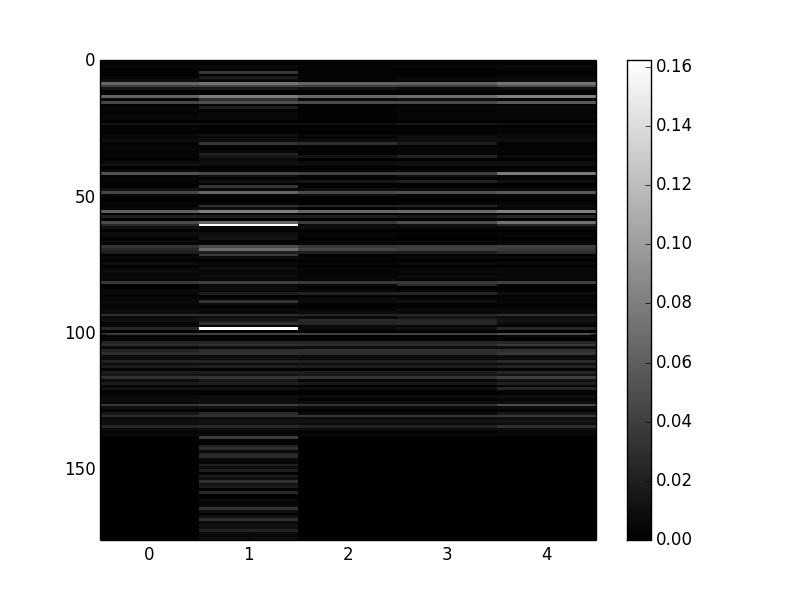
\includegraphics[width=.5\linewidth]{freesurfer-nrmse.png}%
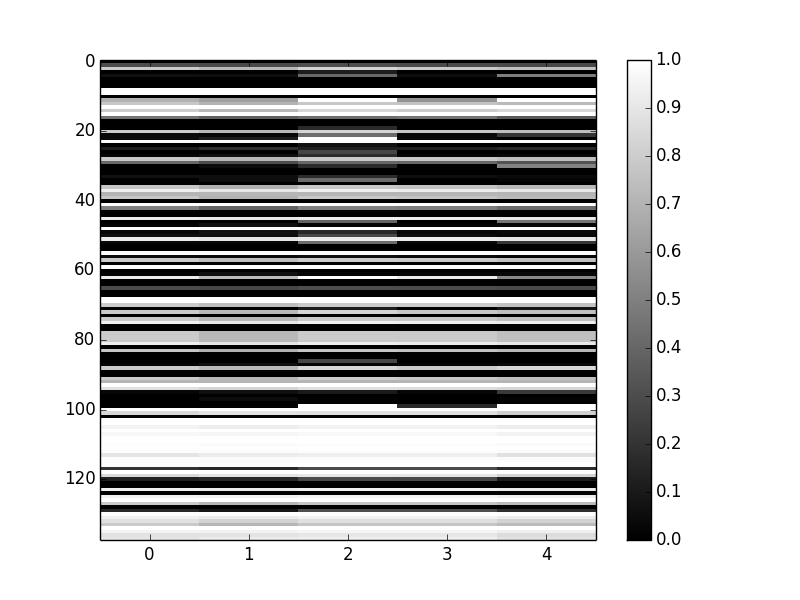
\includegraphics[width=.5\linewidth]{freesurfer-dice.png}
\captionof{figure}{FreeSurfer metric values}
\caption*{(i) NRMSE (left) (ii)Dice Coefficient (right)}
\label{fig:freesurfer_metric_values}
\end{center}

\section{PostFreeSurfer}\label{sec:Postfreesurfer}
25 (.nii.gz) were found to have inter-OS differences after postfreesurfer processing. These files are created as part of PostFreeSurfer processing alone and they are common to all the five subjects. Table~\ref{tab:PostFreeSurfer_Metic_Values} contains the mean, median and standard deviation values of the files having differences across all the subjects.
\hfill \break
\begin{center}
\begin{tabular}{|l|l|l|}
\hline
\textbf{Item}      & \textbf{Nrmse} & \textbf{Dice} \\ \hline
Mean               & 0.03474272     & 0.676874536   \\ \hline
Median             & 0.038619041    & 0.982912774   \\ \hline
Standard Deviation & 0.025485142    & 0.458426209   \\ \hline
\end{tabular}
\captionof{table}{NRMSE \& DICE values for PostFreeSurfer processing on CentOS6 and CentOS7}
\label{tab:PostFreeSurfer_Metic_Values}
\end{center}
\hfill \break

\begin{center}
\begin{longtable}{|p{.3\textwidth}|p{.3\textwidth}|p{.3\textwidth}|}
\cline{1-3}
\textbf{Category} & \textbf{Nrmse} & \textbf{Dice Coeff} \\\cline{1-3}
\multirow{5}{.3\textwidth}{Files consistently different across subjects (low std.dev)}     & \makecell[l]{OrigT1w2standard.nii.gz \\ (xfms)}  & \makecell[l]{wmparc\_1mm.nii.gz\\(T1w)} \\\cline{2-3}
& \makecell[l]{OrigT2w2standard.nii.gz\\(xfms)}                   & \makecell[l]{OrigT2w2standard.nii.gz\\(xfms)} \\\cline{2-3}
& \makecell[l]{OrigT1w2T1w.nii.gz\\(xfms)}                        & \makecell[l]{aparc+aseg.nii.gz\\(T1w)} \\\cline{2-3}
& \makecell[l]{OrigT2w2T1w.nii.gz\\(xfms)}                        & \makecell[l]{aparc.a2009s+aseg.nii.gz\\(T1w)} \\\cline{2-3}
& \makecell[l]{ROIs.2.nii.gz\\(MNINonLinear)}                     & \makecell[l]{OrigT1w2standard.nii.gz\\(xfms)} \\\cline{1-3}
\multirow{5}{.3\textwidth}{Files with differences that vary across subjects (med std. dev)} & \makecell[l]{wmparc.nii.gz\\(T1w)}  & \makecell[l]{T1wDividedByT2w.nii.gz\\(T1w)} \\\cline{2-3}
& \makecell[l]{T2w\_restore.2.nii.gz\\(MNINonlinear)}                       & \makecell[l]{Atlas\_wmparc.2.nii.gz\\(MNINonlinear)} \\\cline{2-3}
& \makecell[l]{wmparc.2.nii.gz\\(MNINonlinear)}                           & \makecell[l]{T1w\_restore.2.nii.gz\\(MNINonlinear)} \\\cline{2-3}
& \makecell[l]{wmparc.nii.gz\\(MNINonlinear)}                      & \makecell[l]{ROIs.2.nii.gz\\(MNINonlinear)} \\\cline{2-3}
& \makecell[l]{brainmask\_fs.nii.gz\\(T1w)}  & \makecell[l]{aparc+aseg.nii.gz\\(MNINonLinear)} \\\cline{1-3}
\multirow{5}{.3\textwidth}{Files with differences that vary specific to each subject (large std. dev)}   & \makecell[l]{aparc+aseg.nii.gz\\(MNINonlinear)}  & \makecell[l]{T2w\_restore.2.nii.gz\\(MNINonLinear)} \\\cline{2-3}
& \makecell[l]{aparc.a2009s\\+aseg.nii.gz\\(T1w)}                              & \makecell[l]{wmparc.nii.gz\\(T1w)} \\\cline{2-3}
& \makecell[l]{aparc.a2009s\\+aseg\_1mm.nii.gz\\(T1w)}                         & \makecell[l]{aparc.a2009s\\+aseg\_1mm.nii.gz\\(T1w)} \\\cline{2-3}
& \makecell[l]{aparc.a2009s\\+aseg.nii.gz\\(MNINonlinear)}                   & \makecell[l]{MNINonLinear\\(wmparc.2.nii.gz)} \\\cline{2-3}
& \makecell[l]{T1wDividedByT2w.nii.gz\\(T1w)}                                & \makecell[l]{aparc.a2009s+aseg.nii.gz\\(MNINonLinear)} \\\cline{1-3}
\end{longtable}
\captionof{table}{NRMSE \& DICE comparison of PostFreeSurfer files with differences on CentOS6 and CentOS7}
\label{tab:PostFreeSurfer_comparison_table}
\end{center}
\hfill \break

\begin{center}
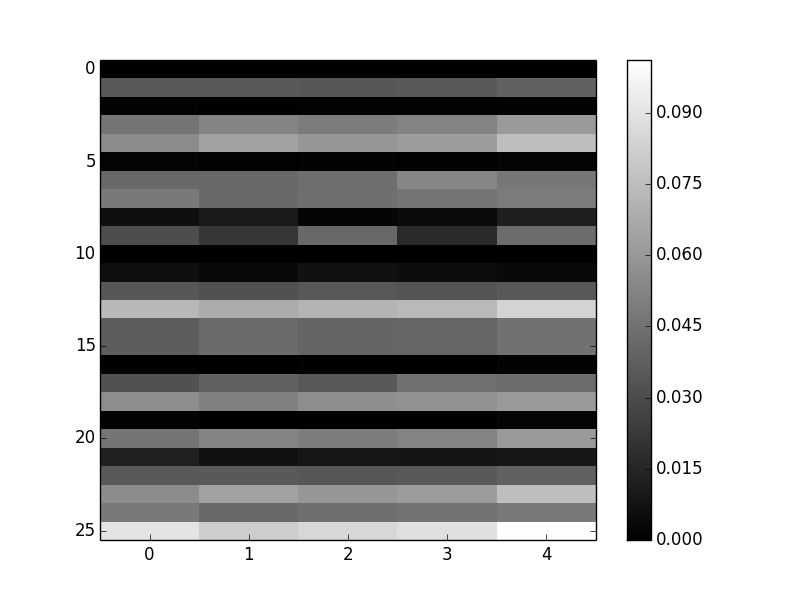
\includegraphics[width=.5\linewidth]{postfreesurfer-nrmse.png}%
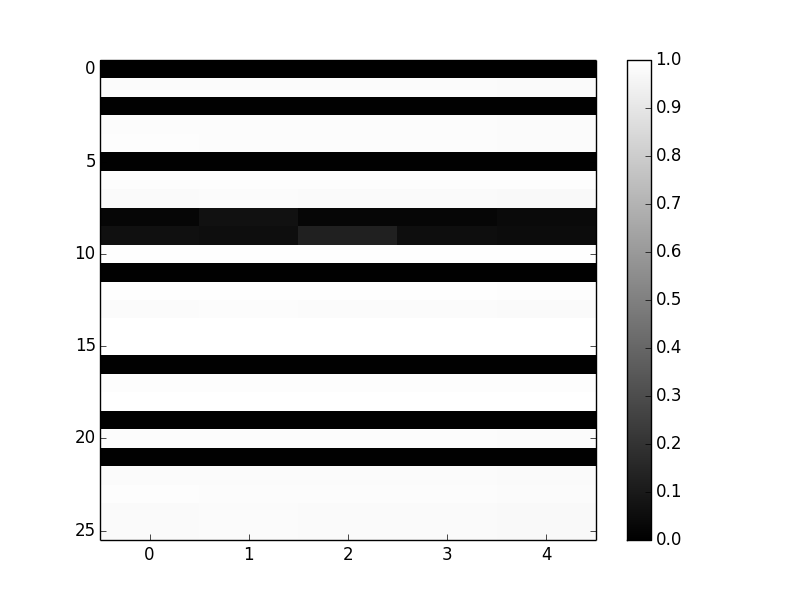
\includegraphics[width=.5\linewidth]{postfreesurfer-dice.png}
\captionof{figure}{PostFreeSurfer metric values}
\caption*{(i) NRMSE (left) (ii)Dice Coefficient (right)}
\label{fig:postfreesurfer_metric_values}
\end{center}

Figure \ref{fig:postfreesurfer_high_nrmse} illustrates the file with the highest NRMSE value out of the postfreesurfer results between CentOS6 and CentOS7. The filename is ``aparc.a2009s+aseg.nii.gz" with the NRMSE value (0.101) from the subject 101410. The red dots in the image shows the differences in the images between two conditions.

\hfill \break
\begin{center}
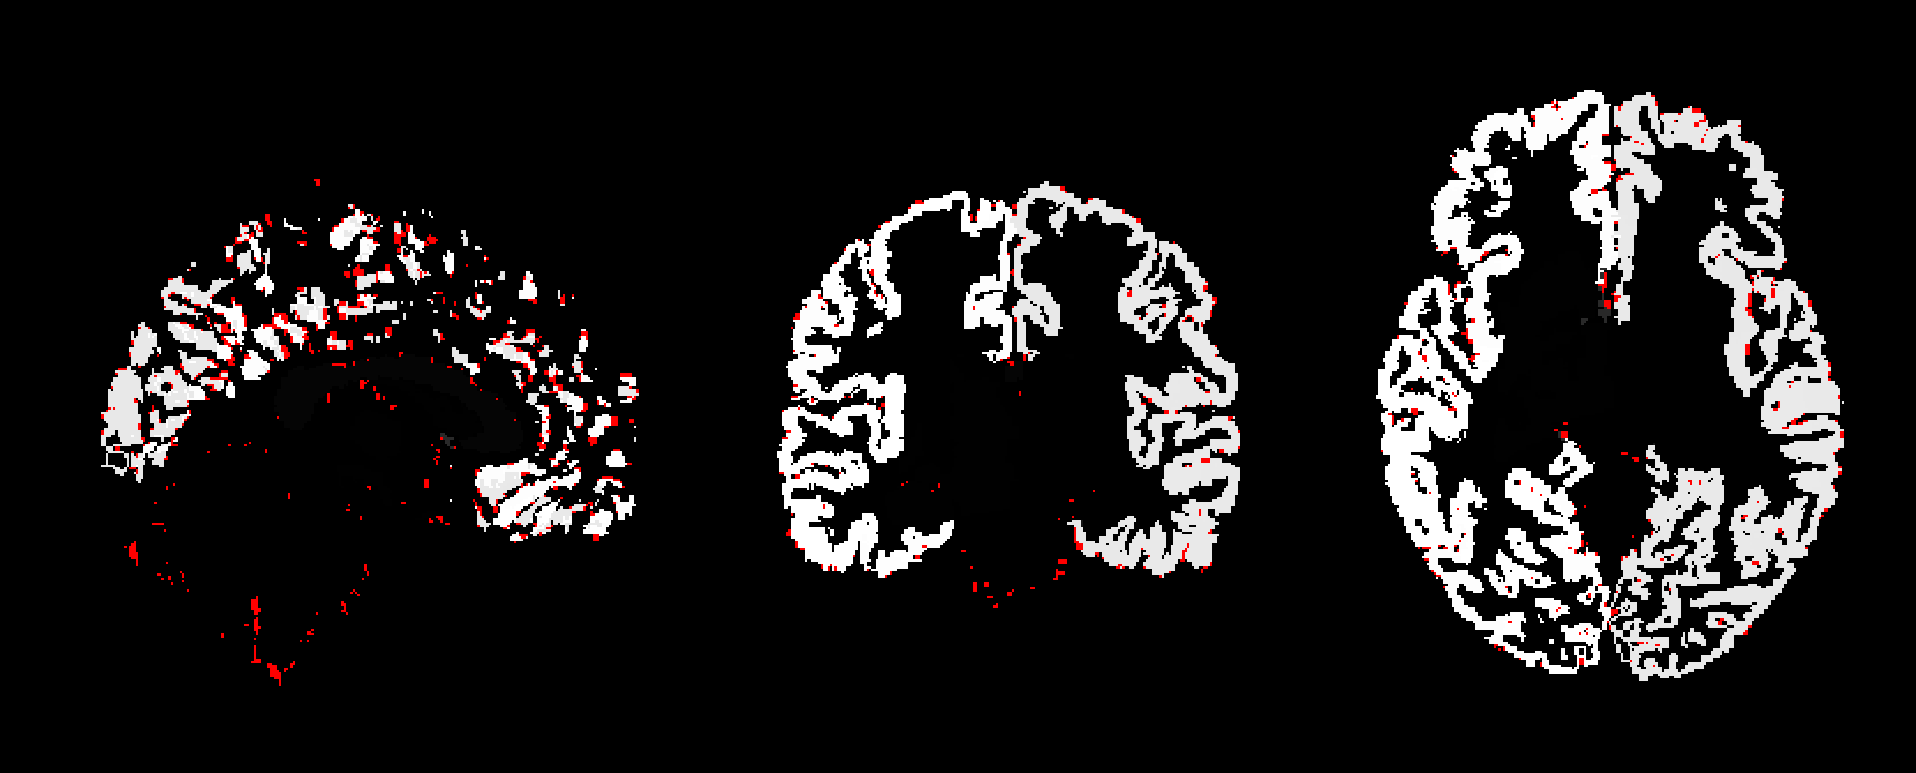
\includegraphics[width=\linewidth]{postfreesurfer-nrmse-aparc-a2009s+aseg.png}
\captionof{figure}{Illustrating the differences in the file with the highest NRMSE value in PostFreeSurfer Processing}
\caption*{(Subject: 101410; Filename: aparc.a2009s+aseg.nii.gz; Dice coeff.: 0.97 ; NRMSE: 0.101)}
\label{fig:postfreesurfer_high_nrmse}
\end{center}

\section{fMRIVolume}\label{sec:fMRI}
1152 files were found to have inter-OS differences after fMRIVolume processing which were common to all subjects. Table~\ref{tab:fMRIVolume_Metric_Values} contains the mean, median and standard deviation values of the files having differences after fMRIVolume processing.
\hfill \break
\begin{center}
\begin{tabular}{|l|l|l|}
\hline
\textbf{Item}      & \textbf{Nrmse}  & \textbf{Dice} \\ \hline
Mean               & 0.016025213     & 0.560550964   \\ \hline
Median             & 0.009066946     & 0.751177948   \\ \hline
Standard Deviation & 0.019648208     & 0.376997518   \\ \hline
\end{tabular}
\captionof{table}{NRMSE \& DICE values for fMRIVolume processing on CentOS6 and CentOS7}
\label{tab:fMRIVolume_Metric_Values}
\end{center}
\hfill \break

\begin{center}
\begin{longtable}{|p{.3\textwidth}|p{.3\textwidth}|p{.3\textwidth}|}
\cline{1-3}
\textbf{Category} & \textbf{Nrmse} & \textbf{Dice Coeff} \\\cline{1-3}
\multirow{5}{.3\textwidth}{Files consistently different across subjects (low std.dev)}     & \makecell[l]{tfMRI\_WM\_RL\_mc\\\_mask.nii.gz \\ (MotionCorrection)}  & \makecell[l]{T1w\_restore.2.nii.gz\\(OneStepResampling)} \\\cline{2-3}
& \makecell[l]{tfMRI\_SOCIAL\_RL\\\_mc\_mask.nii.gz\\(MotionCorrection)}                   & \makecell[l]{tfMRI\_LANGUAGE\\\_RL2standard.nii.gz\\(MNINonLinear)} \\\cline{2-3}
& \makecell[l]{SBRef2PhaseTwo\\\_gdc.nii.gz\\(Fieldmap)}                        & \makecell[l]{Scout\_gdc\_MNI\\\_warp.nii.gz\\(OneStepResampling)} \\\cline{2-3}
& \makecell[l]{SBRef\_dc\_jac.nii.gz\\(Fieldmap)}                        & \makecell[l]{standard2tfMRI\\\_LANGUAGE\_RL.nii.gz\\(xfms)} \\\cline{2-3}
& \makecell[l]{Scout\_gdc\\\_undistorted.nii.gz\\(DistortionCorrection\\AndEPIToT1wReg\\\_FLIRTBBR\\AndFreeSurfer\\BBRbased)}                     & \makecell[l]{Scout\_gdc\_undistorted\\2T1w\_init\_warp.nii.gz\\(DistortionCorrection\\AndEPIToT1wReg\\\_FLIRTBBR\\AndFreeSurfer\\BBRbased)} \\\cline{1-3}
\multirow{5}{.3\textwidth}{Files with differences that vary across subjects (med std. dev)} & \makecell[l]{tfMRI\_MOTOR\_LR\\\_nonlin.nii.gz\\(tfMRI\_MOTOR\_LR)}  & \makecell[l]{tfMRI\_EMOTION\_RL\\\_dropouts.nii.gz\\(ComputeSpin\\EchoBiasField)} \\\cline{2-3}
& \makecell[l]{tfMRI\_GAMBLING\_LR\\\_PhaseOne\_gdc\_dc.nii.gz\\(MNINonlinear)}                       & \makecell[l]{tfMRI\_WM\_LR\\\_dropouts.nii.gz\\(MNINonLinear)} \\\cline{2-3}
& \makecell[l]{sebased\_reference\_dil.nii.gz\\(ComputeSpin\\EchoBiasField)}                           & \makecell[l]{fMRI\_RELATIONAL\_LR\\\_dropouts.nii.gz\\(MNINonLinear)} \\\cline{2-3}
& \makecell[l]{tfMRI\_MOTOR\_LR\\\_PhaseOne\_gdc\_dc.nii.gz\\(MNINonlinear)}                      & \makecell[l]{tfMRI\_GAMBLING\\\_LR\_dropouts.nii.gz\\(MNINonlinear)} \\\cline{2-3}
& \makecell[l]{brainmask\_fs.nii.gz\\(T1w)}  & \makecell[l]{tfMRI\_GAMBLING\\\_RL\_dropouts.nii.gz\\(T1w)} \\\cline{1-3}
\multirow{5}{.3\textwidth}{Files with differences that vary specific to each subject (large std. dev)}   & \makecell[l]{Scout\_gdc\\\_undistorted2T1w\\\_init\_fast\\\_wmedge.nii.gz\\(DistortionCorrection\\AndEPIToT1wReg\\\_FLIRTBBRAnd\\FreeSurferBBRbased)}  & \makecell[l]{tfMRI\_MOTOR\\\_LR\_mc.nii.gz\\(tfMRI\_MOTOR\_LR)} \\\cline{2-3}
& \makecell[l]{SE\_BCdivGRE\\\_brain.nii.gz\\(ComputeSpin\\EchoBiasField)}                            & \makecell[l]{Scout\_gdc\\\_undistorted.nii.gz\\(DistortionCorrection\\AndEPIToT1wReg\\\_FLIRTBBRAnd\\FreeSurferBBRbased)} \\\cline{2-3}
& \makecell[l]{SEdivGRE.nii.gz\\(ComputeSpinEcho\\BiasField)}                         & \makecell[l]{SBRef\_dc\_jac.nii.gz\\(FieldMap)} \\\cline{2-3}
& \makecell[l]{SEdivGRE.nii.gz\\(ComputeSpinEcho\\BiasField)}                         & \makecell[l]{SBRef2PhaseOne\\\_gdc.nii.gz\\(FieldMap)} \\\cline{2-3}
& \makecell[l]{tfMRI\_MOTOR\_LR\_mc\\\_mask.nii.gz\\(MotionCorrection)}               & \makecell[l]{WarpField.nii.gz\\(DistortionCorrection\\AndEPIToT1wReg\\\_FLIRTBBRAnd\\FreeSurferBBRbased)} \\\cline{1-3}
\end{longtable}
\captionof{table}{NRMSE \& DICE comparison of fMRIVolume files with differences on CentOS6 and CentOS7}
\label{tab:fMRIVolume_comparison_table}
\end{center}
\hfill \break

\begin{center}
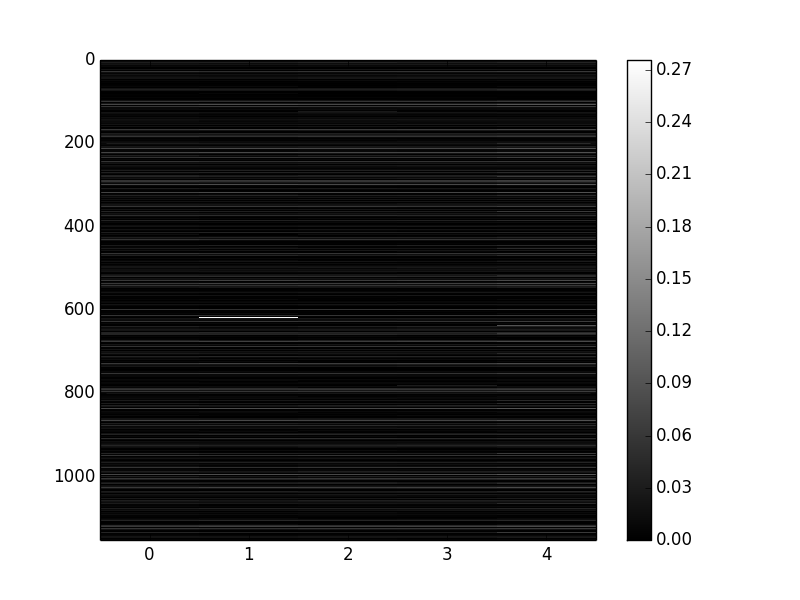
\includegraphics[width=.5\linewidth]{fmri_NRMSE.png}%
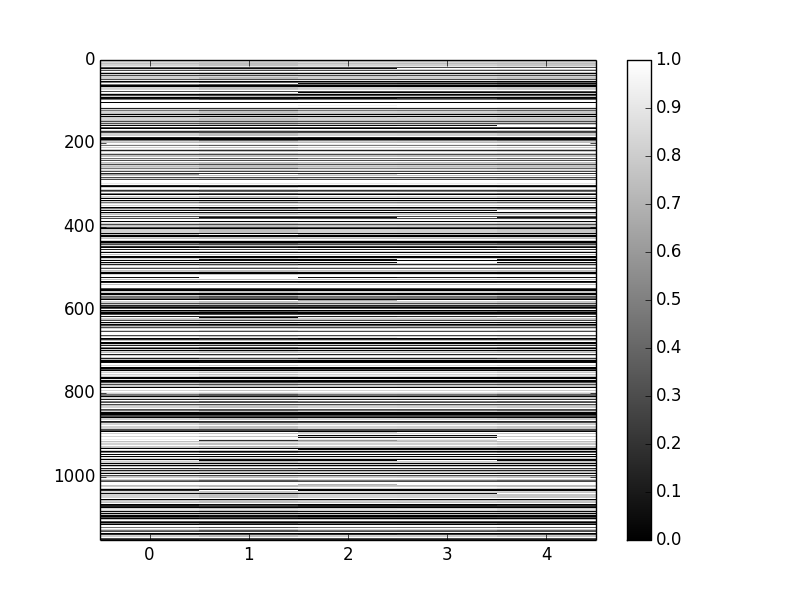
\includegraphics[width=.5\linewidth]{fmri_DICE.png}
\captionof{figure}{fMRIVolume metric values}
\caption*{(i) NRMSE (left) (ii)Dice Coefficient (right)}
\label{fig:fMRI_metric_values}
\end{center}

\hfill \break
\begin{center}
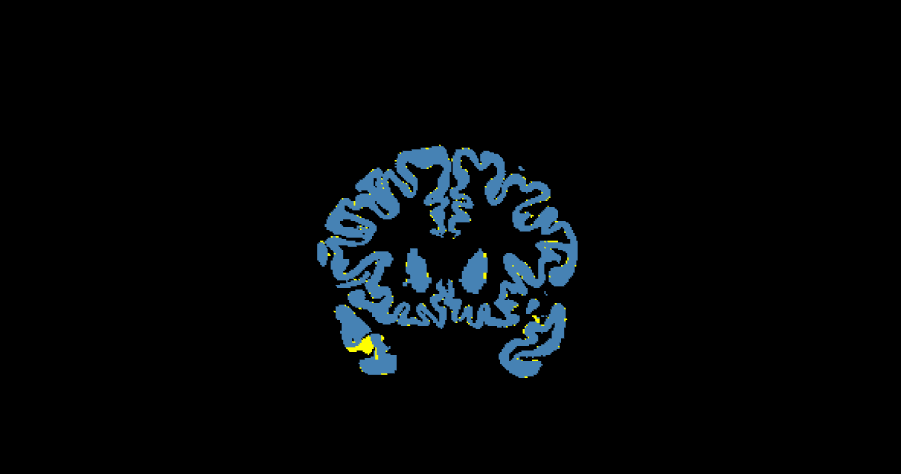
\includegraphics[width=.75\linewidth]{Frontview2.png}%
\captionof{figure}{All Grey Matter file visualizatoin (Blue shaded region shows the CentOS 6 output and yellow region shows the CentOS 7 output).}
\caption*{(Subject: 101006; Filename: AllGreyMatter.nii.gz; Dice coeff.; 0.99; NRMSE; .074)}
\label{fig:allgrey_matter} 
\end{center}

\begin{center}
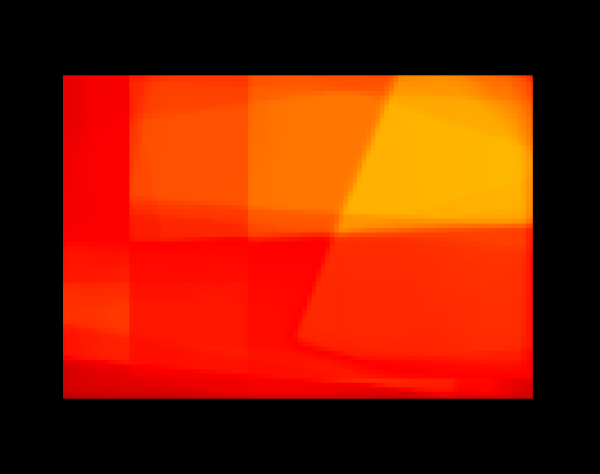
\includegraphics[width=.5\linewidth]{tfMRI_MOTOR_LR_mc_mask_centos6.png}%
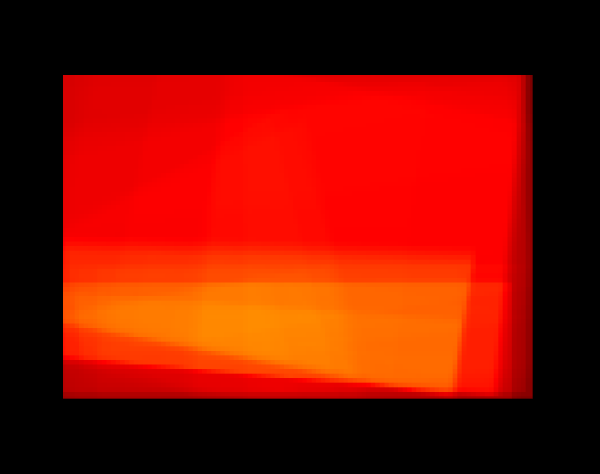
\includegraphics[width=.5\linewidth]{tfMRI_MOTOR_LR_mc_mask_centos7.png}
\captionof{figure}{tfMRI Mask file}
\caption*{(i) tfMRI\_MOTOR\_LR\_mc\_mask.nii.gz file from CentOS6(left) (ii) tfMRI\_MOTOR\_LR\_mc\_mask.nii.gz file from CentOS7}
\label{fig:tfMRI_mask_file}
\end{center}

\section{Effect of changing Subject Vs. changing Condition}\label{sec:comparison}
In order to quantify the effect of operating system on the output image and to compare the difference with the anatomical differences between subjects, we made a comparison with subjects processed in the same condition (two subjects processed in the same condition) vs. the same subjects processed in two different conditions. Subjects 101107 and 101006 processed using PreFreeSurfer on CentOS7 was compared against 101006,101007 processed on (CentOS6 and CentOS7). Table \ref{tab:comparison_table} contains the mean, median and std. deviation across the said conditions.

\hfill \break
\begin{center}
\begin{tabularx}{.99\textwidth}{|c|c|c|c|c|c|c|}
\hline
Item  & \makecell[l]{NRMSE\\(Between\\subjects)} & \makecell[l]{Dice Coeff.\\(Between\\subjects)} & \makecell[l]{NRMSE\\101006\\CentOS\\(6Vs7)} & \makecell[l]{Dice Coeff.\\ 101006\\CentOS\\(6Vs7)} & \makecell[l]{NRMSE\\101107\\CentOS\\(6Vs7)} & \makecell[l]{Dice Coeff.\\ 101107\\CentOS\\(6Vs7)} \\ \hline
Average            & 0.092        & .265      & 0.0066     & 0.3014   & .0077   & .3001     \\ \hline
Median             & 0.078    & .0109       & 0.004          & 0.0217           & .0045     & .021  \\ \hline
\makecell[l]{Std.\\Dev} & 0.073     & 0.377           & 0.0092         & 0.3898   & .0100       & .385 \\ \hline
\end{tabularx}
\captionof{table}{Comparison: Anatomical differences vs. Effect of operating system}
\label{tab:comparison_table}
\end{center}
